% NOTE:
% latexmk -shell-escape -pvc poster.tex # Watches and compiles on each change.
% latexmk -c poster.tex   # Clean the temporal files.


\documentclass[20pt]{beamer}

% Adapted from;
% How to Design a Scientific Poster using Beamer -1 (Latex Basic Tutorial-30)
% https://youtu.be/2ZWnFFhVkdE?si=N3e1Ob8YWyTwW19e

\usepackage[size=custom, width=90, height=120, orientation=portrait, scale=1.4]{beamerposter}
\usetheme{Madrid}
\usepackage{changepage}
\usepackage[numbers]{natbib}
\usepackage{listings}
\usepackage{siunitx}
\usepackage{hyperref}
\usepackage[linesnumbered,algoruled,longend]{algorithm2e}
\usepackage{graphicx}
\usepackage{subcaption}

\beamertemplatenavigationsymbolsempty

\renewcommand{\raggedright}{\leftskip=0pt \rightskip=0pt}
\let\olditemize\itemize
\renewcommand{\itemize}{\olditemize\addtolength{\itemsep}{0.4\baselineskip}}

\addtobeamertemplate{block begin}{}{\vspace{5mm}\begin{adjustwidth}{5mm}{5mm}}
\addtobeamertemplate{block end}{\end{adjustwidth}\vspace{10mm}}{\vspace{5mm}}

\setbeamertemplate{caption}[numbered]

\setbeamerfont{block title}{size={\centering\bfseries\fontsize{48}{60}}}
\setbeamercolor{block body}{bg=white}
\setbeamercolor{background canvas}{bg=white}


\definecolor{rulebg}{RGB}{248,230,0}
\definecolor{titlebg}{RGB}{11,95,156}
\definecolor{titlefontcolor}{RGB}{255,255,255}
\definecolor{rulebg}{RGB}{252,199,21}


\setbeamercolor{fbcolor}{fg=white, bg=titlebg}
\setbeamertemplate{headline}{
    \begin{beamercolorbox}[wd=\paperwidth]{fbcolor}\vskip5mm
        \begin{columns}
            \begin{column}{0.30\linewidth}
            \centering
            
\includegraphics[scale=0.7]{logos/logo_sbsr.png}\\
            \end{column}
            \begin{column}{0.70\linewidth}
                \bfseries
\textcolor{titlefontcolor}{
\fontsize{80pt}{96} 
                \selectfont
                Exploratory analysis of recurrent deforestation \\
                warnings in the Brazilian Amazon\\ [6mm]
{\fontsize{43pt}{60}
                \selectfont 
                Alber Sánchez (alber.ipia@inpe.br), Guilherme Mataveli, Aline Pontes-Lopes,\\
                Sulimar Munira Caparoci Nogueira, and Luiz Arag\~{a}o
}
}
            \end{column}
        \end{columns}
        \vskip 5mm
    \end{beamercolorbox}
    \color{rulebg}\rule{\paperwidth}{20pt}
}

\setbeamercolor{footcolor}{fg=white, bg=black}
\setbeamertemplate{footline}{
\color{rulebg}\rule{\paperwidth}{20pt}
 \begin{beamercolorbox}[wd=\paperwidth]{fbcolor}\vskip5mm
        \begin{columns}
            \begin{column}{0.30\linewidth}
            \centering
            
\includegraphics[scale=2.5]{logos/logoinpe-azul-menor.png}\\
            \end{column}
            \begin{column}{0.40\linewidth}
                \bfseries
\textcolor{titlefontcolor}{
\fontsize{30pt}{96} 
\centering
                \selectfont
                %Acesse o site do grupo:\\ [6mm]
                \vspace{10mm}
                }

\centering
            
\includegraphics[scale=1.8]{logos/trees-color-h_2.png}
                \hspace{10mm}
            
\includegraphics[scale=1.0]{images/qr_treeslab.png}\\
                \vspace{10mm}
            \end{column}
            \begin{column}{0.30\linewidth}
            \centering
            
\includegraphics[scale=1.1]{logos/logo_cnpq.png}\\
            \end{column}
        \end{columns}
    \end{beamercolorbox}
}



\begin{document}\vspace*{-2cm}
\begin{frame}[fragile,t]
\begin{columns}[t]



%==== Column 1 ====

\begin{column}{0.33\linewidth}

\vspace{0.5cm}

    \begin{block}{Introduction\vphantom{g}}
        We believe that DETER, the real-time forest monitoring systems that continuously issues deforestation alerts in the Brazilian Amazon since 2004~\cite{shimabukuro2006}, inadvertently captures forest degradation processes.
        Here we present some of our findings after processing 5 years of DETER alerts.
        This poster extends the results introduced in ~\cite{sanchez2023}.
    \end{block}

\vspace{0.5cm}

    \begin{block}{Data}
        We analyzed DETER data (polygons) from August 2016 to July 2021.
        The total area of DETER alerts have been increasing since 2019, and the area of the largest alerts reached its top in 2017 (Figure~\ref{fig:deter_warnings_area_size}).
        It must be noted that DETER data is not meant for estimating neither deforestation nor degradation but for monitoring and also that it captures only the final stages of the degradation process~\cite{dealmeida2022}.

\begin{figure}[h] 
    \begin{center}
    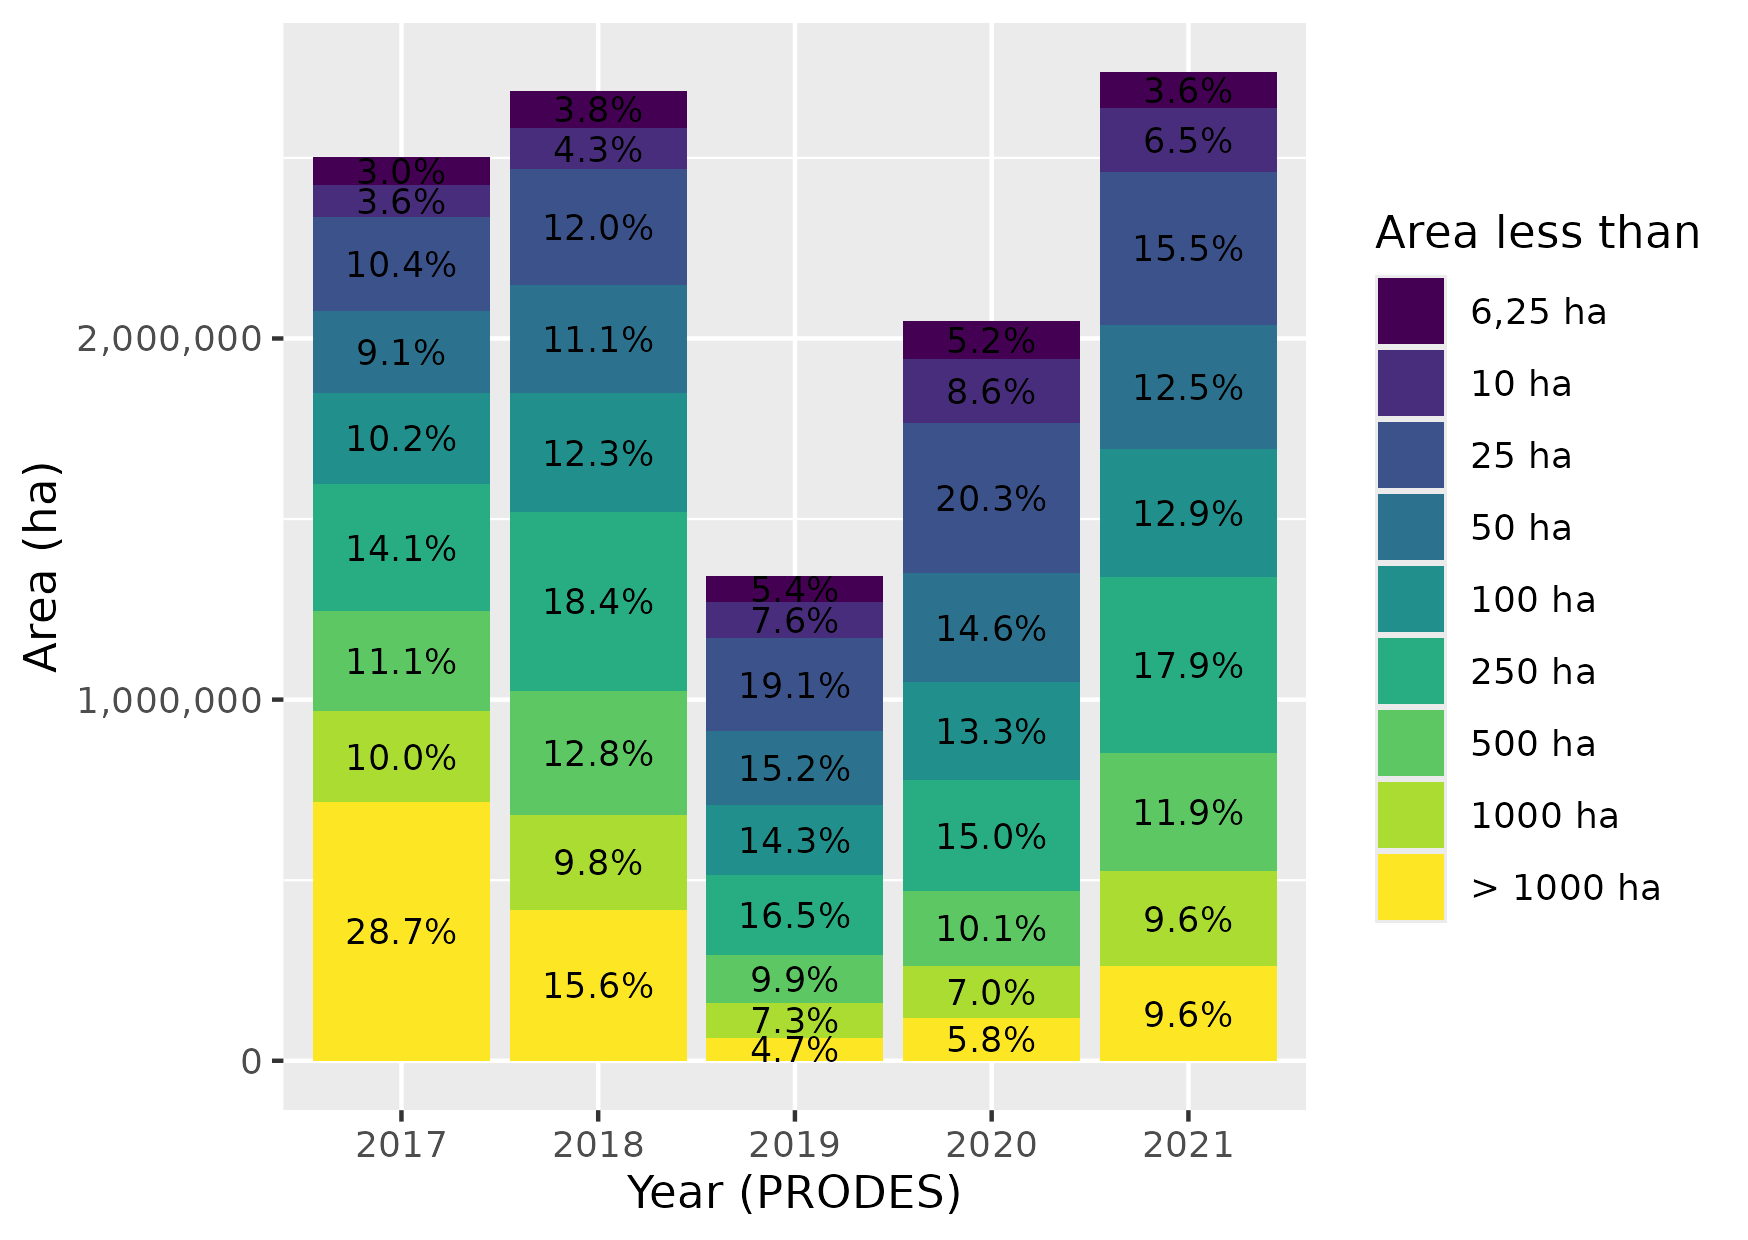
\includegraphics[width=\linewidth]{./figures/deter_warnings_area_size.png}
        \caption{Area of DETER alerts by year and size.}
    \label{fig:deter_warnings_area_size}
    \end{center}
\end{figure}

        However, considering the number of DETER alerts, most of them are issued in on small areas (Figure~\ref{fig:deter_warnings_size}).

\begin{figure}[h] 
    \begin{center}
    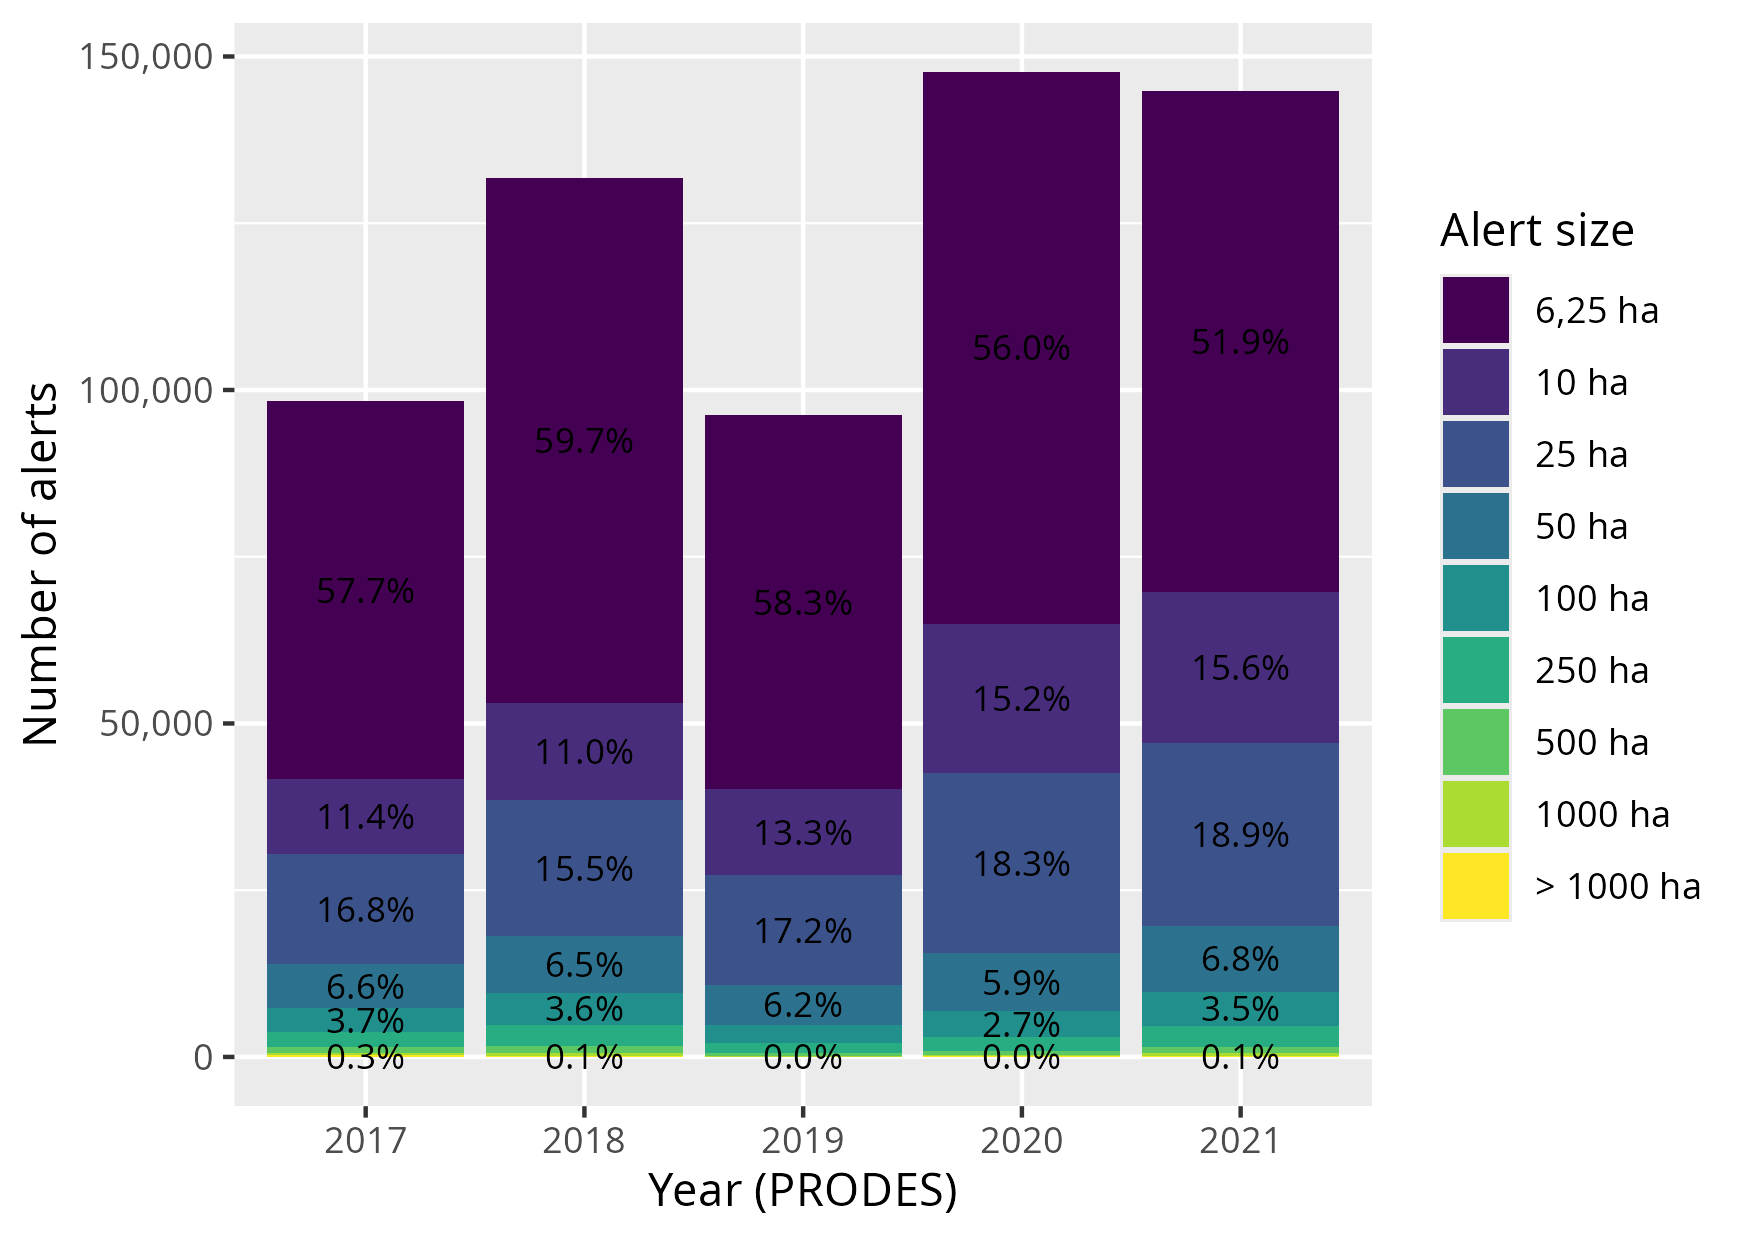
\includegraphics[width=\linewidth]{./figures/deter_warnings_size.png}
    \caption{Number of DETER alerts by year and size.}
    \label{fig:deter_warnings_size}
    \end{center}
\end{figure}

    \end{block}

\vspace{0.5cm}

    \begin{block}{Methods}
        \begin{enumerate}
            \item We downloaded DETER data from the TerraBrasilis~\cite{f.g.assis2019}. 
            \item We computed the PRODES year (August to July).
            \item Then we self-intersected the data, resulting in homogeneous polygons along time that we call subareas.
            \item We projected the data to the coordinate reference system UTM 22s.
            \item We removed duplicated vertices and enforced the right-hand rule for polygons, and fixed geometry errors.
            \item In accordance with DETER method, we removed polygons smaller than 3~ha.
        \end{enumerate}
    \end{block}

\end{column}



%==== Column 2 ====

\begin{column}{0.33\linewidth}

\vspace{0.5cm}

    \begin{block}{Results\vphantom{g}}
        The \textit{subareas} resulting from self-intersecting DETER alerts, which correspond to geometrically consistent polygons at different dates, are the basis of our analysis.

        We found that most of DETER subareas are issued a single alert and never more than five, following an exponential decay pattern and the \textit{subareas} size is similar when aggregated by number of alerts (see Figure~\ref{fig:plot_area_by_warnings}).

\begin{figure}[h] 
    \begin{center}
    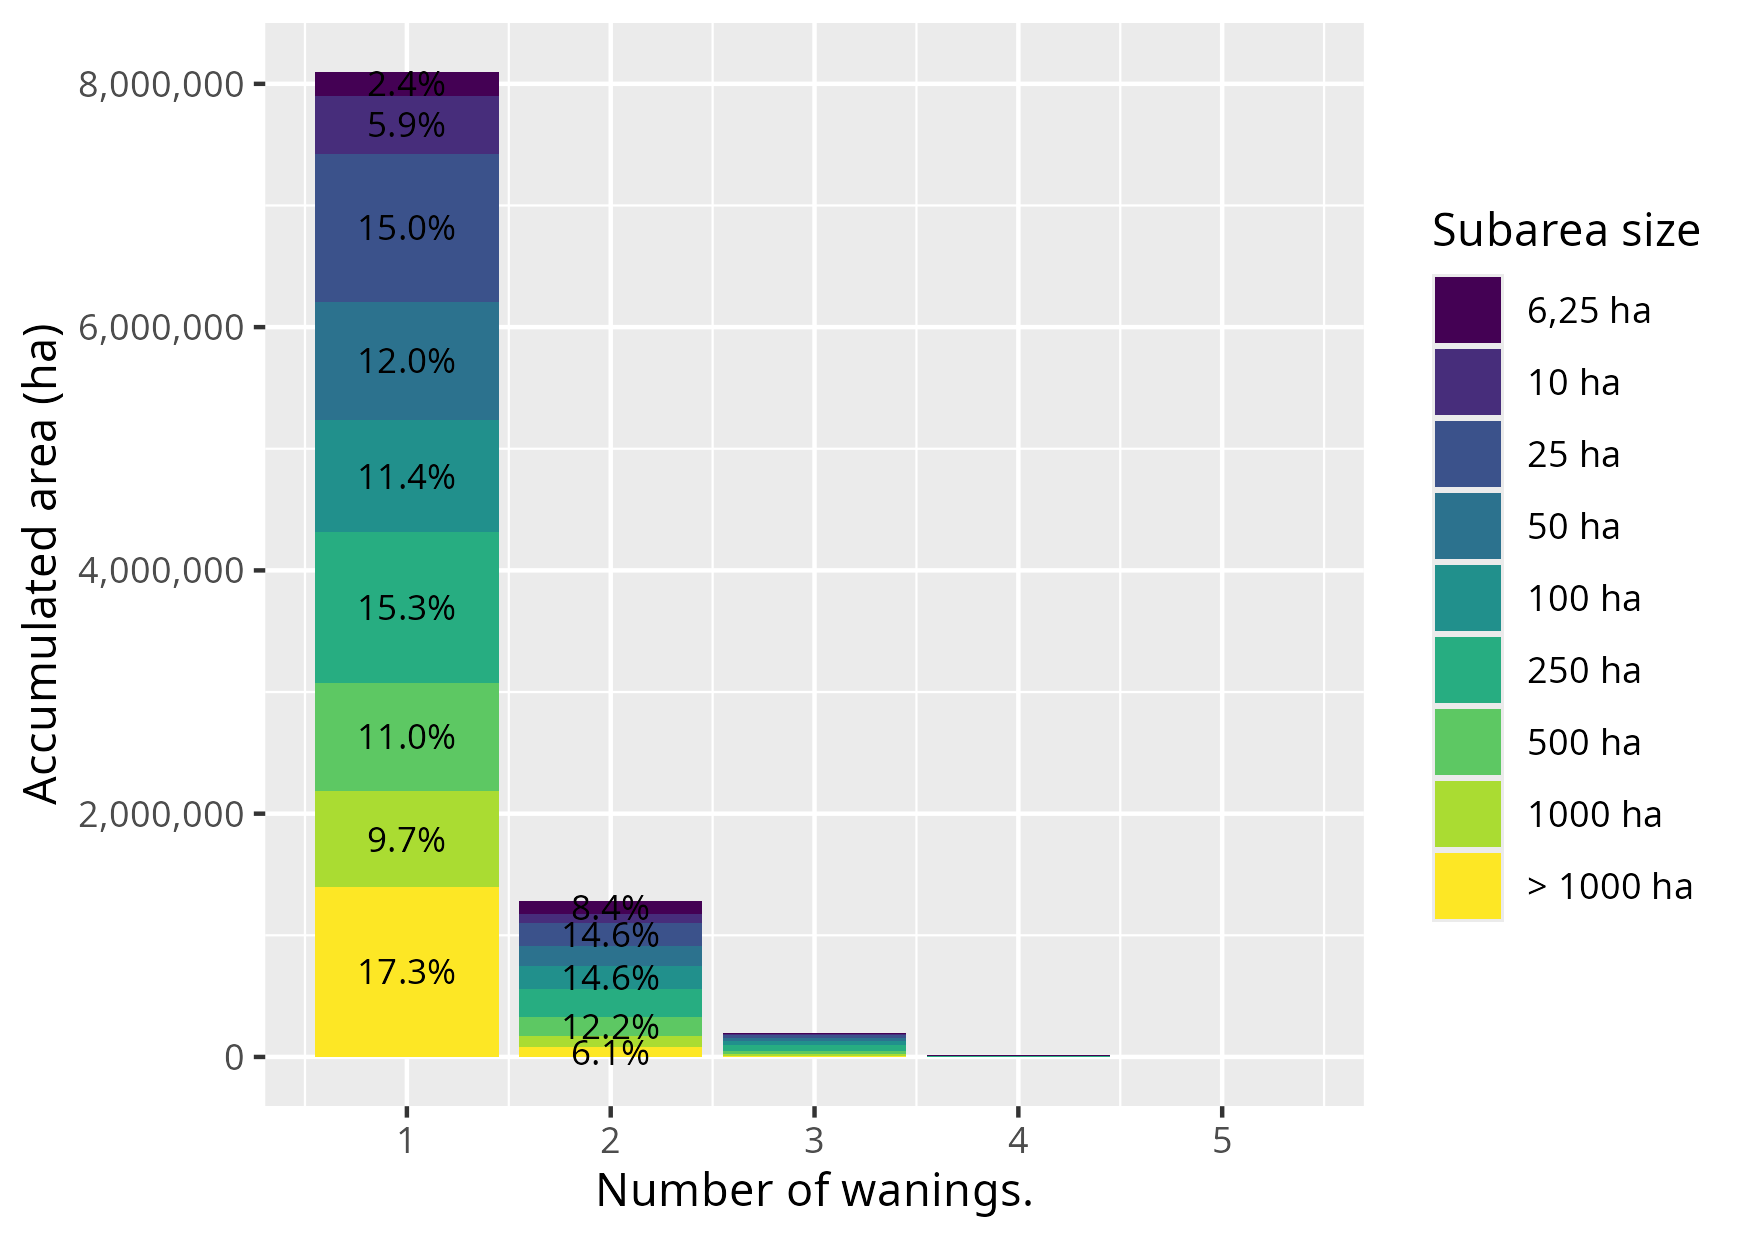
\includegraphics[width=\linewidth]{./figures/plot_area_by_warnings.png}
    \caption{DETER subareas by number of alerts. }
    \label{fig:plot_area_by_warnings}
    \end{center}
\end{figure}

        DETER subareas with 2 warnings tend to be two years apart and then increase one year with each additional alert.
        Also note the trend of longer tails towards longer periods of time (Figure~\ref{fig:plot_days_first_to_last}). 
        This is consistent with DETER's policy of not reviewing the same area more than once during the same year~\cite{dealmeida2022}.

\begin{figure}[h] 
    \begin{center}
        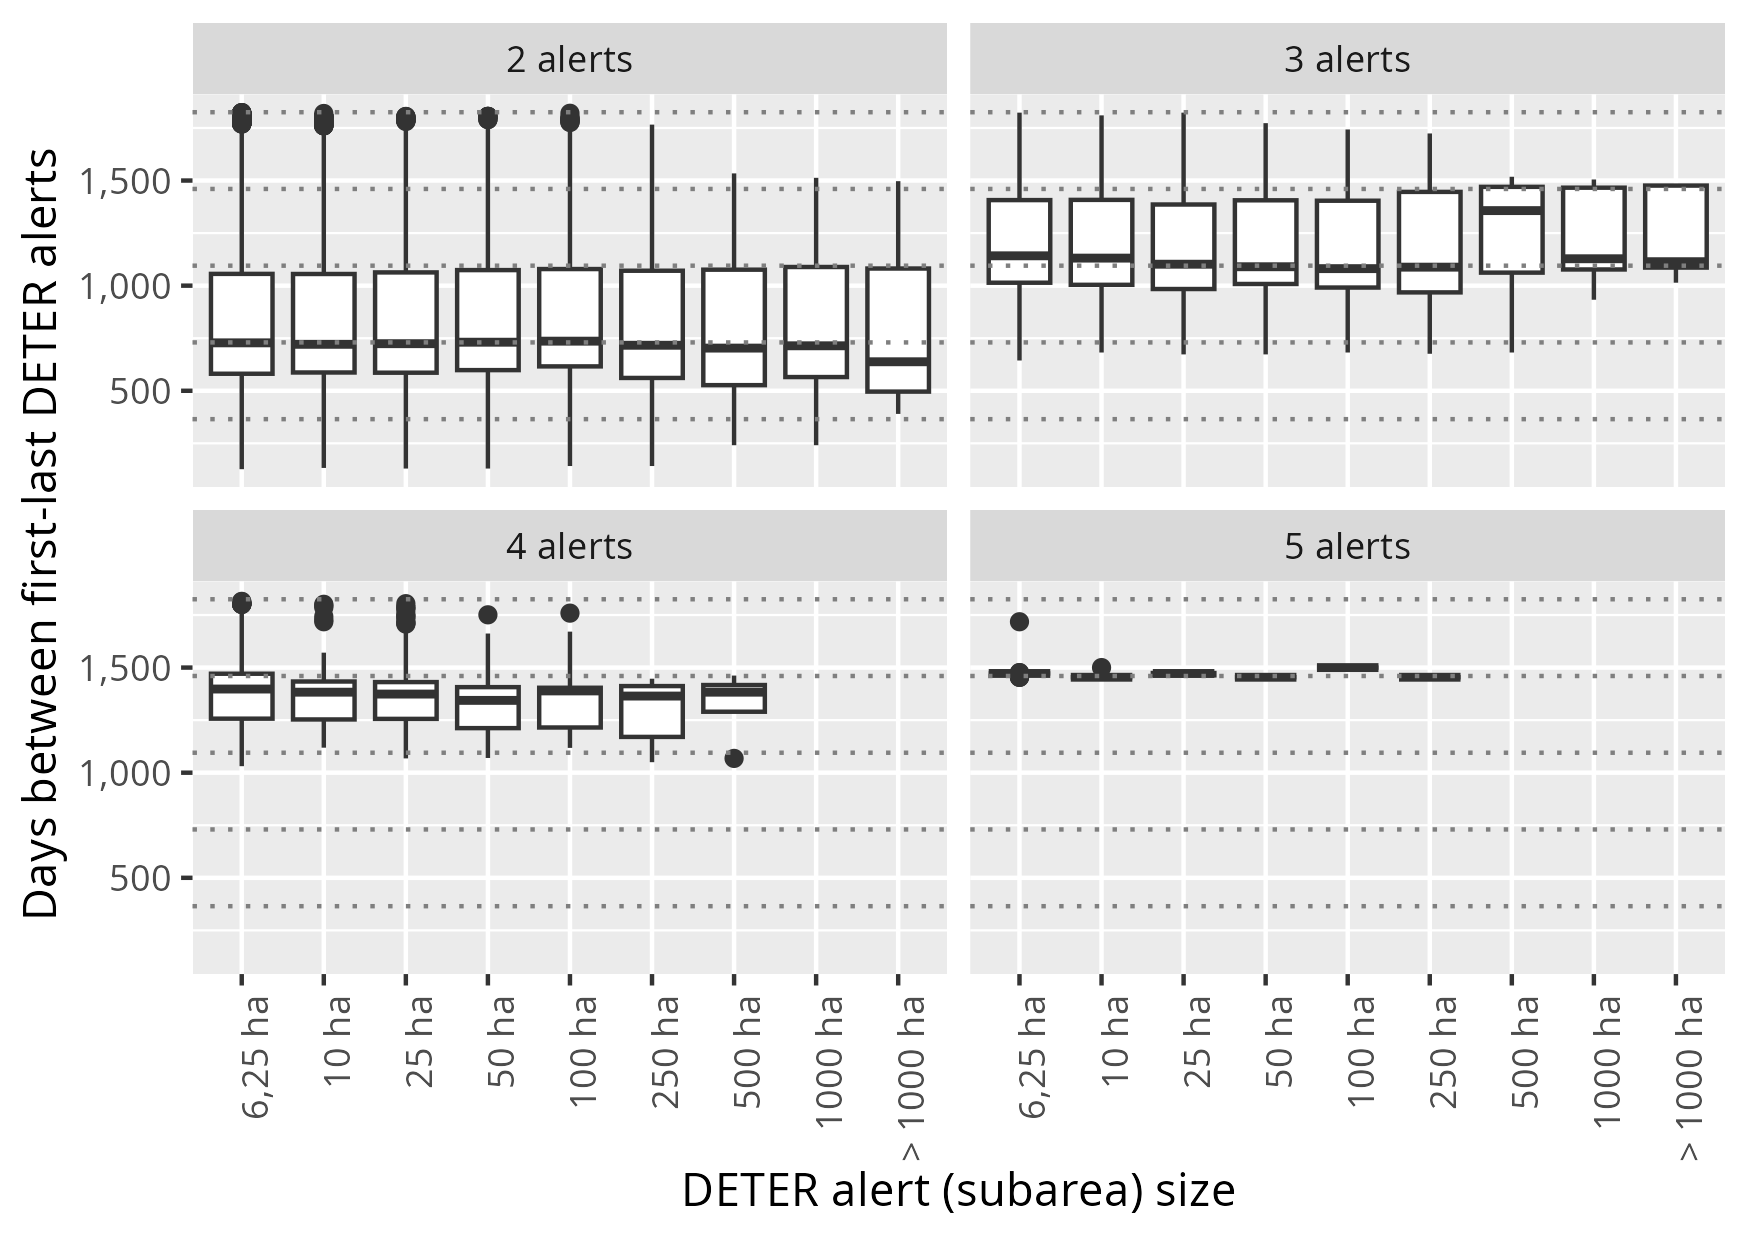
\includegraphics[width=\linewidth]{./figures/plot_days_first_to_last.png}
        \caption{Number of days between the first and last DETER alerts by \textit{subarea} size. The horizontal dashed black lines represent intervals of 365 days.}
    \label{fig:plot_days_first_to_last}
    \end{center}
\end{figure}

        The map in Figure~\ref{fig:plot_area_by_warnings} shows the distribution of recurrent deforestation warnings, that is, a surface interpolation (inverse distance weighting - IDW) of the number of DETER alerts.

\begin{figure}[h] 
    \begin{center}
        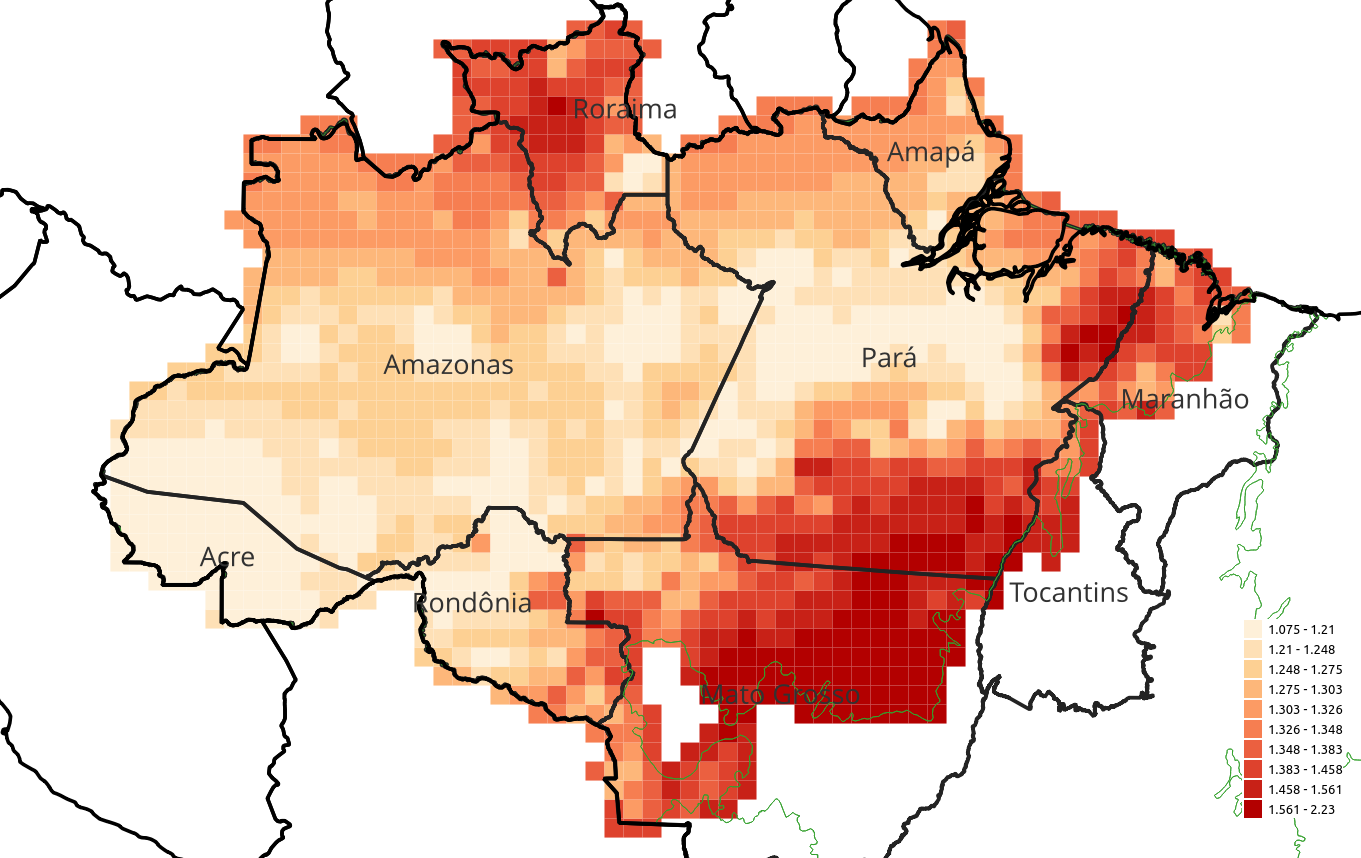
\includegraphics[width=\linewidth]{./figures/nwarnings_idw_map_with_legend.png}
        \caption{Distribution of recurrent degradation (number of
        DETER alerts by subarea) in the Brazilian Amazon. Amazon's east front is
        where most of recurrent DETER alerts area found. Some smoothing is introduced by the interpolation method (IDW).}
    \label{fig:nwarnings_idw_map}
    \end{center}
\end{figure}

\vspace{0.3cm}

    \end{block}
\end{column}

%
%Moreover, the number of DETER alerts during the same period shows a somewhat similar pattern, characterized by the fact that half of yearly DETER alerts are issued for small areas (Figure~\ref{fig:deter_warnings_size}).
%
%From August to October is when most DETER alerts are issued, and September, the peak month, presents an increasing trend in area, reaching its maximum in 2021.
%This period corresponds to the fire season in most of the Brazilian Amazon~\cite{carvalho2021} (see Figure~\ref{fig:deter_warnings_size_month}). 



%==== Column 3 ====

\begin{column}{0.33\linewidth}

\vspace{0.5cm}

    \begin{block}{Final remarks\vphantom{g}}
        \begin{itemize}
            \item Our results show that recurrent DETER alerts over the same area are uncommon, and proportionally inverse to the number of alerts.
            \item They also show that the \textit{subareas} with the most recurrent alerts tend to happen along the east of Amazonia (the deforestation arc) and to the north, in \textit{Roraima} state (Figure~\ref{fig:plot_area_by_warnings} and Figure~\ref{fig:nwarnings_idw_map}).
            \item Also, most of the successive alerts in the same \textit{subarea} are at most five years apart (that is, the duration of our dataset, from 2016 to 2021), two years from the first to the second, and one year from there. 
            \item It must be taken into account that DETER data is produced for a purpose other than the analysis presented here, and that it acknowledges its under estimation of forest degradation due to its associated challenges~\cite{dealmeida2022}.
            \item Our analyses were carried out using the GNU's R language and environment for statistical computing and graphics to estimate statistics analysis~\cite{ihaka1996} and QGIS version 3.38.0~\cite{QGIS_software}. Additionally, our source code is available online (see links below).
        \end{itemize}
    \end{block}

\vspace{1cm}

    \begin{block}{References\vphantom{g}}
        {\small
\bibliography{sbsr2024}
\bibliographystyle{sbc}
        }
    \end{block}

\vspace{0.5cm}

    \begin{block}{Links}
\begin{figure}
    \begin{subfigure}[b]{0.2\textwidth}

\includegraphics[width=0.99\textwidth]{images/qrcode_email_alber_ipia_at_inpe.png} \\
\centering
{Email.}
    \end{subfigure}
    ~
    \begin{subfigure}[b]{0.2\textwidth}

\includegraphics[width=0.99\textwidth]{images/qrcode_prioritizedeforestationhotspots.png} \\
\centering
{Code.}
    \end{subfigure}
    ~
    \begin{subfigure}[b]{0.2\textwidth}

\includegraphics[width=0.99\textwidth]{images/qr_poster.png} \\
\centering
{Poster.}
    \end{subfigure}
\end{figure}
\vspace{0.7cm}
    \begin{itemize}
        \item Email: alber.ipia@inpe.br
        \item Code: {\small\url{https://github.com/albhasan/treesburnareas}}
        \item Poster: {\small\url{https://github.com/albhasan/slides/blob/main/sbsr2024/doc/latex/poster.pdf}}
    \end{itemize}
    \end{block}
\end{column}


\end{columns}
\end{frame}
\end{document}
